\documentclass[border=8pt]{standalone}
\usepackage{pgf-pie}
\usepackage{xcolor}

% Paleta: azules (investigación/diseño), verdes (implementación), naranja (entreno/eval), púrpura (infra/MLOps), gris (redacción)
\definecolor{c1}{RGB}{52,120,190}   % Investigación
\definecolor{c2}{RGB}{90,160,220}   % Diseño arquitectura
\definecolor{c3}{RGB}{34,150,100}   % Pipeline datos
\definecolor{c4}{RGB}{70,180,130}   % Mejoras arquitectónicas
\definecolor{c5}{RGB}{210,120,40}   % Ciclos entrenamiento
\definecolor{c6}{RGB}{230,160,60}   % Evaluación
\definecolor{c7}{RGB}{140,60,180}   % Infraestructura Cloud
\definecolor{c8}{RGB}{180,80,200}   % MLOps
\definecolor{c9}{RGB}{130,130,130}  % Redacción

\begin{document}
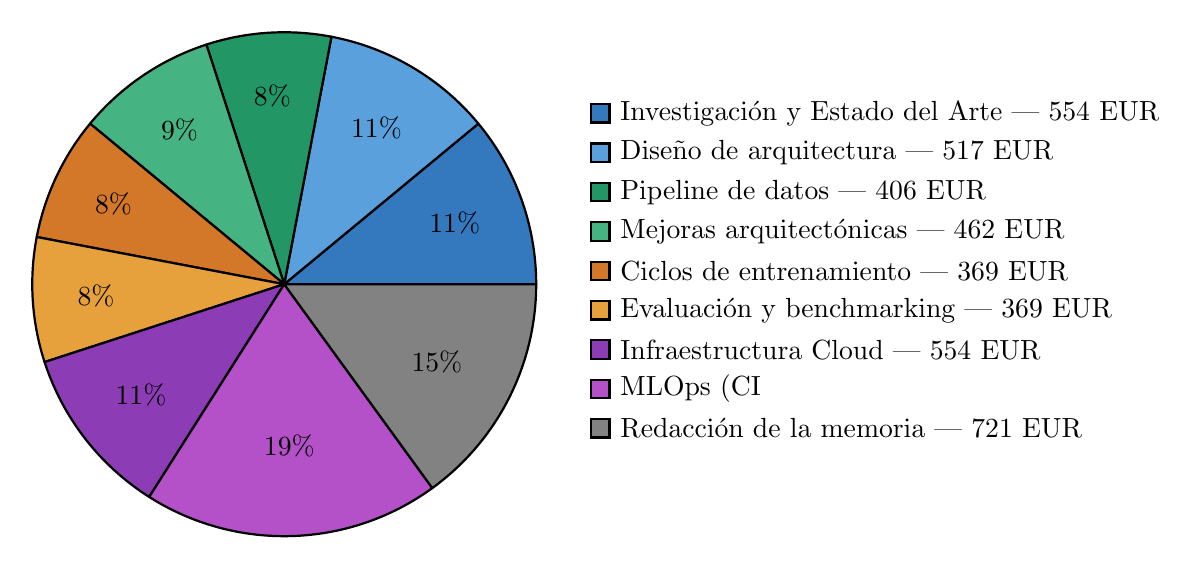
\begin{tikzpicture}
\pie[
    radius=3.2,
    color={c1,c2,c3,c4,c5,c6,c7,c8,c9},
    text=legend,
    after number=\%,
    every label/.style={font=\small}
]{
    11/Investigación y Estado del Arte --- 554 EUR,
    11/Diseño de arquitectura --- 517 EUR,
    8/Pipeline de datos --- 406 EUR,
    9/Mejoras arquitectónicas --- 462 EUR,
    8/Ciclos de entrenamiento --- 369 EUR,
    8/Evaluación y benchmarking --- 369 EUR,
    11/Infraestructura Cloud --- 554 EUR,
    19/MLOps (CI/CD\text{,} Docker\text{,} K8s) --- 924 EUR,
    15/Redacción de la memoria --- 721 EUR
}
\end{tikzpicture}
\end{document}
